\section{Evaluation}
\label{evaluation}
\noindent
To evaluate the accuracy of our modeling framework, we used a cluster of 6 nodes and used Xen hypervisor \cite{xen} to create up to four virtual machines on each physical machine. Each virtual machine is configured with 4GB of memory and 1 CPU core. For the deployed Apache Spark platform, one machine serves as the master node, and the remaining five machines serve as working nodes. In six physical machines, we create multiple clusters leveraging virtual machines to execute multiple Apache Spark jobs in parallel. 
\noindent
In our evaluation, for prediction, first, we need to estimate the parameter $\beta_{n}$ in equation (\ref{beta}). Towards that, we implemented our own Apache Spark job and executed that on our cluster to obtain the execution time and resource consumption information. This simulation job consists of three stages executing distinct(), groupByKey(), and count() operation respectively. Distinct() implements a mapping function and parses the input data, groupByKey() processes the output of distinct() operation, and count() is a CPU intensive operation performing data summarization. This simulation job is executed with 2.5 GB of sample data where the first stage implementing the Distinct() operation involves significant I/O compared to the following two stages. To measure $\beta_{n}$, we executed $n$ ($n$=1,2,3,4) instances of this simulation job in parallel. As shown in Figure \ref{simjobs}, the effect of interference is significant for the first stage but minimal for the subsequent stages. 
\begin{figure}[!t]
\centering
\captionsetup{justification=centering}
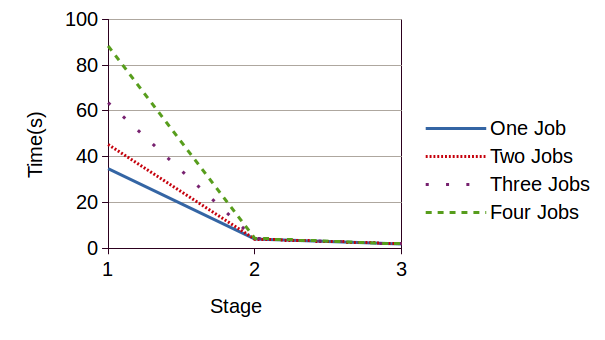
\includegraphics[width=3in]{figures/simjobs.png}
\caption{Execution Time for Different Number of Simulation Jobs}
\label{simjobs}
\end{figure}
\noindent
Once we estimate the value of $\beta_{n}$, subsequently, we used our formulation to predict the execution time for each stage for each job separately in different execution scenarios and add up the prediction error for each stage to calculate the total prediction accuracy $R$ as below.
\begin{equation}
\label{predictaccuracy}
R = |1 - \sum_{i=1}^{M} \frac{|PredictedTime_i - MeasuredTime_i|}{\sum_{j=1}^{M} Time_{j}}|
\end{equation}
\noindent
Here $M$ is the number of stages in a job, $PredictedTime_i$ is the predicted execution time for $stage_i$, and $MeasuredTime_i$ is the actual execution time of $stage_i$. Different evaluation scenarios are presented below.



\subsection{Interference Among Multiple Jobs of the Same Type Starting Simultaneously}
\noindent
In this part of the evaluation, we present the accuracy of prediction while modeling the effect of interference among multiple jobs of the same type (e.g., interference between n instances of job x). Towards that, we choose four Apache Spark jobs: PageRank, K-Means, Logistic Regression and WordCount. WordCount job is a non-iterative job while the remaining three are iterative jobs. For PageRank, we use the LiveJournal network dataset from SNAP \cite{snap}, which is processed through mapping each node id into longer string to form a 20 GB input data set. K-Means and Logistic Regression applications use 20 GB of numerical Color-Magnitude Diagram data of galaxy from Sloan Digital Sky Survey (SDSS) \cite{sdss}. WordCount application uses 20 GB of Wikipedia dump data.
\begin{table}[!t]
\renewcommand{\arraystretch}{1.3}
\caption{Prediction Accuracy for Interference Among Same Jobs}
\label{table_samejob}
\centering
\begin{tabular}{c|c|c|c}
\hline
\bfseries JobName & \bfseries Job Number & \bfseries First Stage & \bfseries Whole Job\\
\hline\hline
PR & 2 & 0.97 & 0.80\\
& 3 & 0.96 & 0.85\\
& 4 & 0.92 & 0.82\\
\hline
KM & 2 & 0.75 & 0.70\\
& 3 & 0.71 & 0.68\\
& 4 & 0.98 & 0.92\\
\hline
LR & 2 & 0.74 & 0.78\\
& 3 & 0.79 & 0.81\\
& 4 & 0.97 & 0.97 \\
\hline
WC & 2 & 0.87 & 0.86\\
& 3 & 0.96 & 0.94\\
& 4 & 0.95 & 0.94\\
\hline
\end{tabular}
\end{table}
\noindent
For prediction, we first executed the sample job (e.g., Page rank) with 2.5 GB of input data to collect the job execution profile, which is then used to predict the execution time assuming no interference. Finally, we used our framework to adjust the prediction assuming interference. The prediction accuracy is summarized in Table~\ref{table_samejob}. In the table, PR, KM, LR, and WC refers to PageRank, K-Means, Logistic Regression, and WordCount application respectively. Column Job number (e.g., 2, 3, 4) indicates the number of jobs that were executed in parallel. For instance, a value of 2 indicates that two instances of the same job were executed in parallel. As can be seen, prediction accuracy is highest for Logistic regression application (97\%) and lowest for K-means (68\%).The predicted execution time and the actual execution time when we executed four instances of the same job in parallel are shown in Figure~\ref{pr20gprIII}, Figure~\ref{km20gkmIII}, Figure~\ref{lr20glrIII}, and Figure~\ref{wc20gwcIII} for PageRank, K-Means, Logistic Regression, and WordCount respectively. 
\begin{figure}[!t]
\centering
\captionsetup{justification=centering}
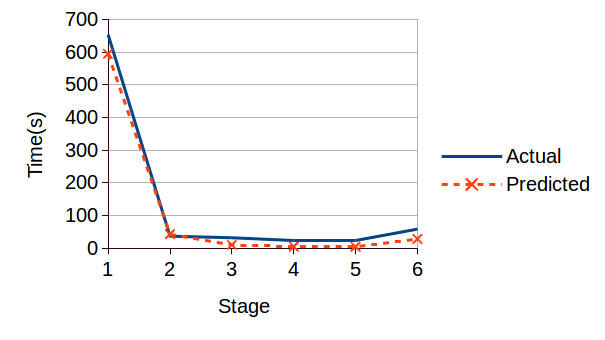
\includegraphics[width=3in]{figures/pr20g_prIII.png}
\caption{Execution Time Prediction for Four Interfered PageRank Jobs}
\label{pr20gprIII}
\end{figure}
\begin{figure}[!t]
\centering
\captionsetup{justification=centering}
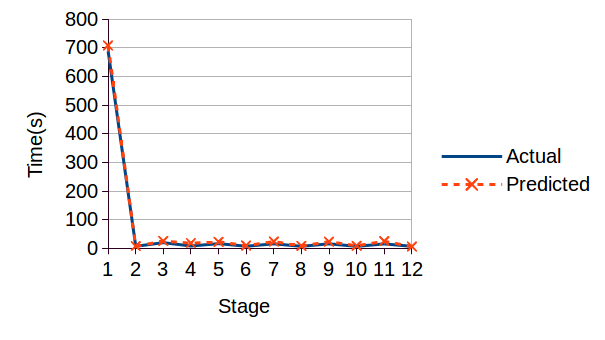
\includegraphics[width=3in]{figures/km20g_kmIII.png}
\caption{Execution Time Prediction for Four Interfered K-Means Jobs}
\label{km20gkmIII}
\end{figure}
\begin{figure}[!t]
\centering
\captionsetup{justification=centering}
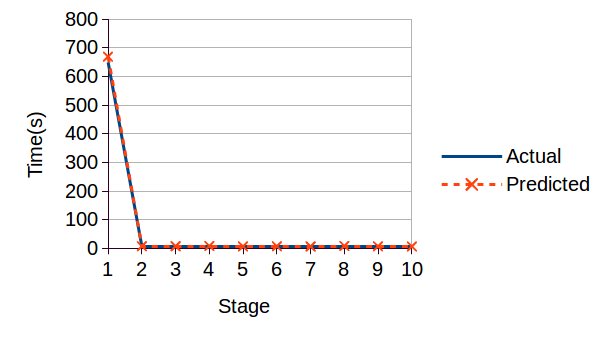
\includegraphics[width=3in]{figures/lr20g_lrIII.png}
\caption{Execution Time Prediction for Four Interfered Logistic Regression Jobs}
\label{lr20glrIII}
\end{figure}
\begin{figure}[!t]
\centering
\captionsetup{justification=centering}
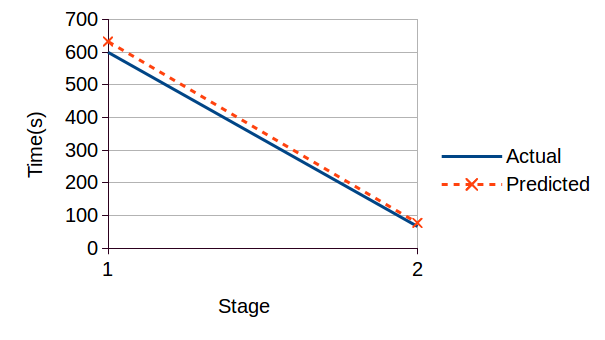
\includegraphics[width=3in]{figures/wc20g_wcIII.png}
\caption{Execution Time Prediction for Four Interfered WordCount Jobs}
\label{wc20gwcIII}
\end{figure}
\noindent


\subsection{Interference Among Multiple Jobs of Different Types Starting Simultaneously}
\noindent
In this section, we present the accuracy of prediction while modeling the interference among $n$ different jobs concurrently, where $n$ was varied between 2 to 4. For example, when $n$ = 2, we execute two different jobs concurrently. The prediction accuracy while running two different jobs in parallel is summarized in Table~\ref{table_twojobs}. As shown in the table, there are a total of 6 combinations to consider. As can be seen, prediction accuracy ranges between 97\% and 69\% for the whole job, and between 99\% and 70\% for the first stage, which incurs the bulk of the execution time. 
\noindent
For $n$=3, we execute three different jobs concurrently. The prediction accuracy while running three different jobs in parallel is summarized in Table~\ref{table_threejobs}. As shown in the table, there are a total of 4 combinations to consider. As can be seen, prediction accuracy ranges between 90\% and 79\% for the whole job, and between 99\% and 83\% for the first stage.
\noindent
Finally, for $n$=4, we execute four different jobs concurrently. The prediction accuracy while running four different jobs in parallel is summarized in Table~\ref{table_fourjobs}. As shown in the table, there are a total of 1 combination to consider. As can be seen, prediction accuracy ranges between 99\% and 86\% for the whole job, and between 99\% and 92\% for the first stage.
\begin{table}[!t]
\renewcommand{\arraystretch}{1.3}
\caption{Prediction Accuracy for Two Different Jobs}
\label{table_twojobs}
\centering
\begin{tabular}{c|c|c|c}
\hline
\bfseries JobName & \bfseries Interfered Job & \bfseries First Stage & \bfseries Whole Job\\
\hline\hline
PR & KM & 0.91 & 0.79\\
& LR & 0.93 & 0.81\\
& WC & 0.99 & 0.85\\
\hline
KM & PR & 0.89 & 0.80\\
& LR & 0.80 & 0.73\\
& WC & 0.75 & 0.69\\
\hline
LR & PR & 0.97 & 0.97 \\
& KM & 0.73 & 0.77\\
& WC & 0.70 & 0.75\\ 
\hline
WC & PR & 0.96 & 0.87\\
& KM & 0.93 & 0.84\\
& LR & 0.96 & 0.88\\
\hline
\end{tabular}
\end{table}
\begin{table}[!t]
\renewcommand{\arraystretch}{1.3}
\caption{Prediction Accuracy for Three Different Jobs}
\label{table_threejobs}
\centering
\begin{tabular}{c|c|c|c}
\hline
\bfseries JobName & \bfseries Interfered Jobs & \bfseries First Stage & \bfseries Whole Job\\
\hline\hline
PR & KM, LR & 0.96 & 0.87\\
& KM, WC & 0.99 & 0.90\\
& LR, WC & 0.99 & 0.90\\
\hline
KM & PR, LR & 0.84 & 0.79\\
& PR, WC & 0.92 & 0.87\\
& LR, WC & 0.83 & 0.80\\
\hline
LR & PR, KM & 0.84 & 0.85\\
& PR, WC & 0.87 & 0.88\\
& KM, WC & 0.83 & 0.84\\
\hline
WC & PR, LR & 0.93 & 0.87\\
& PR, KM & 0.93 & 0.87\\
& KM, LR & 0.94 & 0.89\\
\hline
\end{tabular}
\end{table}
\begin{table}[!t]
\renewcommand{\arraystretch}{1.3}
\caption{Prediction Accuracy for Four Different Jobs}
\label{table_fourjobs}
\centering
\begin{tabular}{c|c|c|c}
\hline
\bfseries JobName & \bfseries Interfered Jobs & \bfseries First Stage & \bfseries Whole Job\\
\hline\hline
PR & KM, LR, WC & 0.92 & 0.86\\
\hline
KM & PR, LR, WC & 0.99 & 0.95\\
\hline
LR & PR, KM, WC & 0.99 & 0.99 \\
\hline
WC & PR, KM, LR & 0.95 & 0.90\\
\hline
\end{tabular}
\end{table}
The predicted execution time and the actual execution time when we executed four different jobs in parallel are shown in Figure~\ref{pr20gkmlrwc}, Figure~\ref{km20gprlrwc}, Figure~\ref{lr20gprkmwc}, and Figure~\ref{wc20gprkmlr} for PageRank, K-Means, Logistic Regression, and WordCount respectively. 
\begin{figure}[!t]
\centering
\captionsetup{justification=centering}
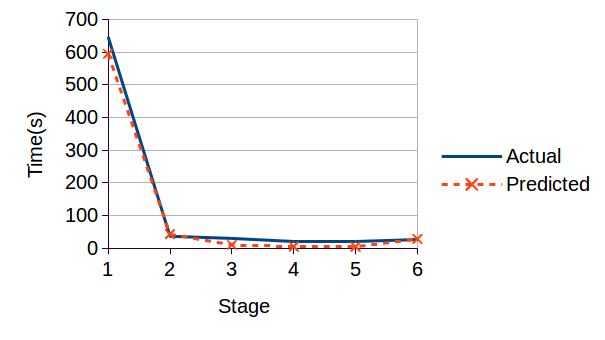
\includegraphics[width=3in]{figures/pr20g_km_lr_wc.png}
\caption{Execution Time Prediction for PageRank Job Interfered with Other Three Jobs}
\label{pr20gkmlrwc}
\end{figure}
\begin{figure}[!t]
\centering
\captionsetup{justification=centering}
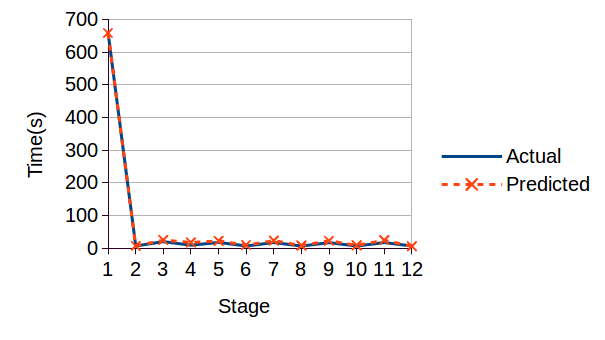
\includegraphics[width=3in]{figures/km20g_pr_lr_wc.png}
\caption{Execution Time Prediction for K-Means Job Interfered with Other Three Jobs}
\label{km20gprlrwc}
\end{figure}
\begin{figure}[!t]
\centering
\captionsetup{justification=centering}
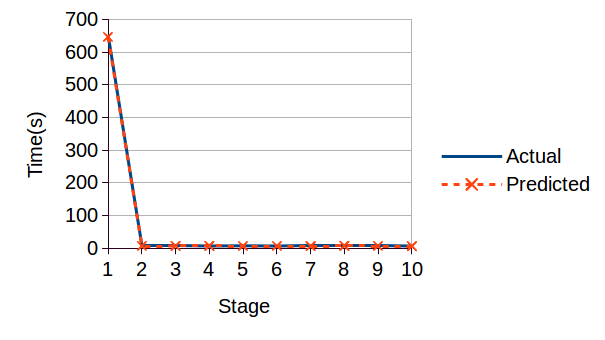
\includegraphics[width=3in]{figures/lr20g_pr_km_wc.png}
\caption{Execution Time Prediction for Logistic Regression Job Interfered with Other Three Jobs}
\label{lr20gprkmwc}
\end{figure}
\begin{figure}[!t]
\centering
\captionsetup{justification=centering}
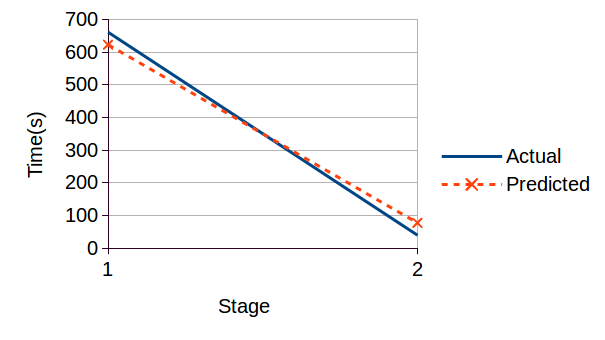
\includegraphics[width=3in]{figures/wc20g_pr_km_lr.png}
\caption{Execution Time Prediction for WordCount Job Interfered with Other Three Jobs}
\label{wc20gprkmlr}
\end{figure}

